\chapter{Digital Video Interface}
\gls{dvi} is a video interface which surfaced in 1999. Designed by the \gls{ddwg} as a replacement for \gls{vga}, it was mainly used to display output from a computer's graphics adapter onto a monitor, although it did see some limited use in other entertainment equipment such as televisions and DVD players. Despite its age, the interface has more than enough bandwidth for 1080p RAW video and its relative simplicity makes it an attractive base for transferring image sensor data.

\section{Interface overview}

In \gls{dvi} nomenclature, a \gls{dvi} link is comprised of an input and output video stream, and the corresponding \gls{tmds} circuitry which is used to transmit the video from one side of a link to the other. Figure \ref{fig:dvi_link_overview} illustrates a typical single-link, consisting of a transmitter / receiver pair joined by four serial \gls{tmds} channels. In the standard RGB operating mode, the three colour components (red, green and blue) are separated and transmitted one per channel, with the remaining channel being used to carry the pixel clock. In addition to pixel data, each channel also has two bits for control signals. On the blue channel (channel 0), the control lines are used to carry the horizontal and vertical synchronisation signals needed for data recovery at the receiver. All other control lines are reserved for future use.

\begin{figure}
  \centering
  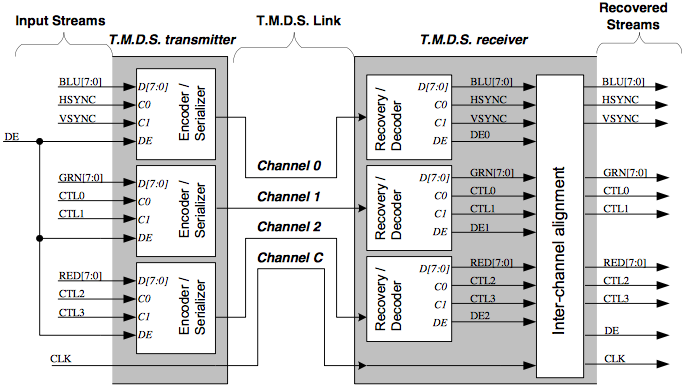
\includegraphics[width=1\textwidth]{./img/dvi_link_overview.png}\par
Source: DVI 1.0 Specification
  \caption{Single \gls{dvi} link in RGB mode.}
  \label{fig:dvi_link_overview}
\end{figure}

\subsection{Video format and timing}

Unlike other modern digital video interfaces, \gls{dvi} does not packetise its data for transmission. Instead, it uses a legacy raster scan technique which was originally intended to drive the electron gun inside a \gls{crt} display. While raster scanning is redundant for digital displays, \gls{dvi} opts for this technique in order to ensure backwards compatibility with the \gls{vga} interface, which was originally designed for use with analogue \gls{crt} displays.

\begin{figure}
  \centering
  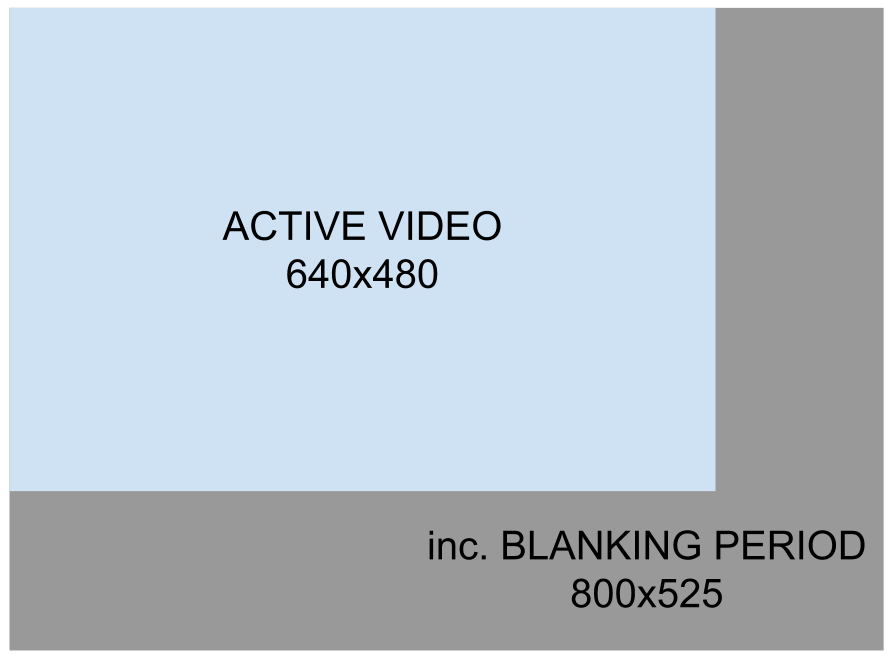
\includegraphics[width=1\textwidth]{./img/raster_scan.png}
  \caption{Illustration of visible pixels and blanking periods.}
  \label{fig:raster_scan}
\end{figure}

\begin{figure}
  \centering
  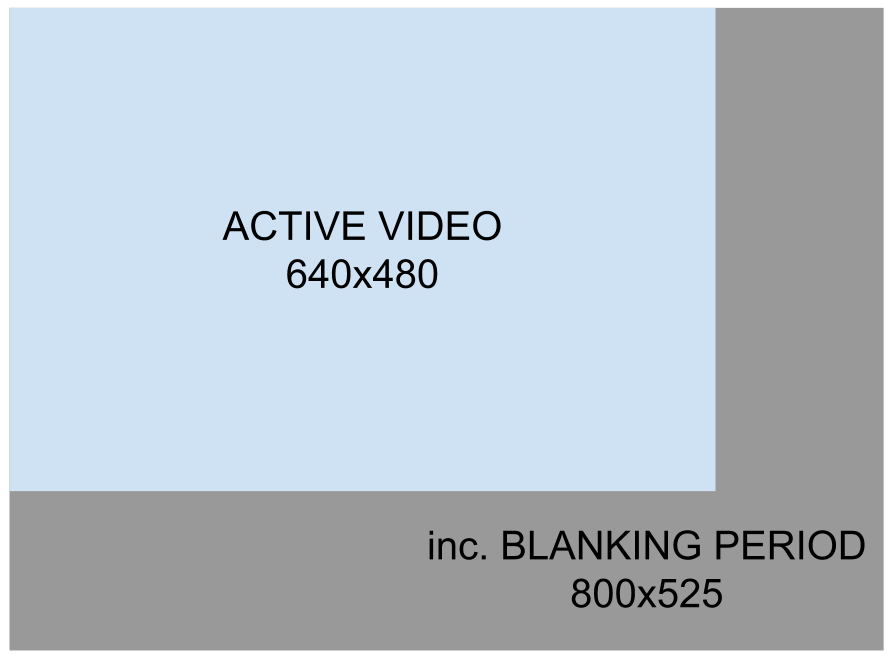
\includegraphics[width=1\textwidth]{./img/raster_scan.png}
  \caption{Video timing synchronisation signals used to mark end of line (HSYNC) and end of frame (VSYNC).}
  \label{fig:video_timing_signals}
\end{figure}

Figures \ref{fig:raster_scan} illustrate the raster scan video technique. If this image was displayed on a monitor, only the blue 'active video' part would be visible, while the grey 'blanking period' extends beyond the display and thus is not drawn, rather it is used to carry the timing signals in Figure \ref{fig:video_timing_signals}. In an analogue monitor these signals would have been used to position the electron beam, however in modern digital displays the HSYNC (end of line) and VSYNC (end of frame) signals are used to detect the video resolution. A list of common video timings can be found in Table.\marginpar{Need to add a table for this}. Single-link \gls{dvi} requires all devices to support a colour-depth of 24-bits per pixel. Unlike \gls{hdmi}, which supports both RGB and YUV data formats, \gls{dvi} only supports RGB.

\subsection{Physical layer}

\gls{dvi} utilises \gls{tmds} in order to reduce \gls{emi}, improve noise immunity and increase skew tolerance for driving data through longer cables. Although the proof-of-concept presented here utilises a cable to link the sensor module and image processor together, noise immunity and skew tolerance are not particularly useful as a real commercial system would use a board-to-board connector to mate the two systems directly together. As mentioned in the overview, a \gls{tmds} link consists of three completely separate data channels and a clock channel. Because of the colour component separation, all three channels are functionally identical and can operate independently of each other; though the clock channel is required for synchronisation.

Like most other high-speed serial interfaces, \gls{tmds} utilises a line coding scheme in order to ensure low \gls{emi}, better noise immunity and skew tolerance. The function of the \gls{tmds} encoder is to take the parallel 8-bit pixel value and 2-bit control data, and convert them into a 10-bit character which may utilise these attributes. Figure \ref{fig:dvi_link_overview} illustrates how the red, green and blue channels are fed into the corresponding encoders (all of which are functionally identical) to produce three serial streams of 10-bit \gls{tmds} characters. Only pixel data or control data may be transmitted at any one time, and so an additional data input signal is required to determine whether the 10-bit \gls{tmds} character is produced from the pixel data (\texttt{DE = 1}) or the control data (\texttt{DE = 0}). 

In order to reduce the number of transitions (and thus the \gls{emi}), the encoder uses a special algorithm for pixel data which produces characters with no more than five transitions, however control data characters use a different algorithm which can produce over seven transitions, though the relatively short duration of the blanking period ensures this is not an issue. Despite all three channels being referenced to the same pixel clock, there is a high chance of the three channels being out of phase at the receiver as a result of trace-length mismatches and various other factors which introduce signal skewing. For the receiver to function correctly, all input channels need to be phase-aligned. To aid this, the \gls{tmds} encoder produces long runs of similar characters which can be easily detected by the receiver in order to mark character boundaries and align the channels.

\gls{tmds} is a serial protocol, and thus the 10-bit output characters from the encoder are serialised and transmitted alongside a \gls{tmds} reference clock. While increasing the maximum bandwidth, serial transition also reduces cost and complexity, allowing a minimal \gls{dvi} interface to be implemented using only four wires. Unlike some high-speed serial interfaces, the clock does not need to be recovered from the data as it is transmitted alongside it. Every clock cycle the \gls{tmds} transmitter outputs a 10-bit character.

\subsection{DDC and EDID}

Alongside the \gls{tmds} signals, \gls{dvi} also includes an I\textsuperscript{2}C-based \gls{ddc} interface for communication between the graphics host and display device. While variants of \gls{ddc} exist which allow for complex heirarchies of devices and bidirectional communication, \gls{dvi} only requires DDC2B to be implemented.

The DDC2B interface allows for a graphics host and display device to be connected in a master / slave configuration, with the graphics host always designated as bus master. As the interface is based on the I\textsuperscript{2}C protocol, each slave must be assigned an address so that other devices can talk to it. In DDC2B the slave is assigned address \texttt{0xA0} (\texttt{0xA0} for writes, \texttt{0xA1} for reads). Figure \ref{fig:i2c_bus} shows a simple master / slave configuration.

\begin{figure}
  \centering
  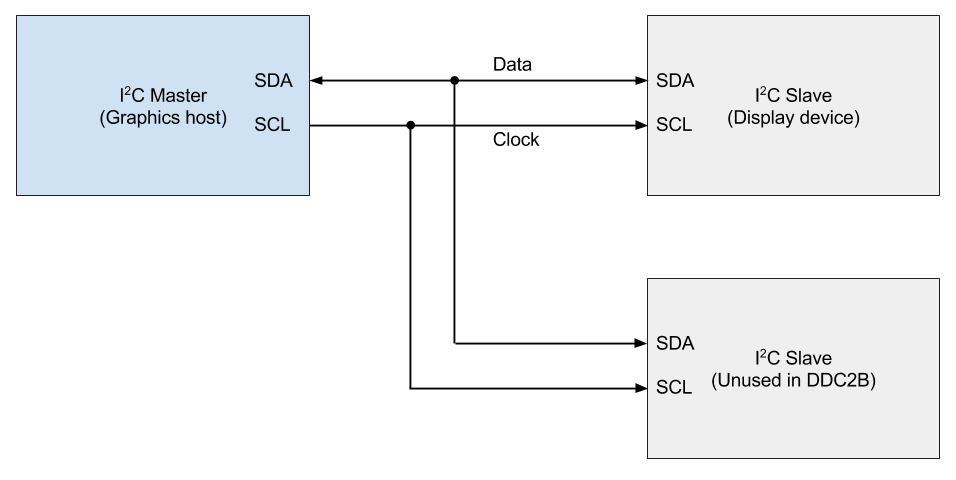
\includegraphics[width=1\textwidth]{./img/i2c_bus.png}
  \caption{A typical I\textsuperscript{2}C master / slave configuration. DDC2B specifies a single master (graphics host) and a single slave (display device).}
  \label{fig:i2c_bus}
\end{figure}

I\textsuperscript{2}C requires only two nets, regardless of the number of master and slave devices, thus it is a very simple and cost effective protocol. I\textsuperscript{2}C messages are one of two types: address frames and data frames. When the master wants to read data data from a slave, it sends out a frame with the address of the slave followed by a data frame containing any additional information (such as a specific register to read), the slave then responds with a data frame containing the requested data.

\gls{edid} is a standardised data structure which may be used by a display device to describe various capabilities such as supported resolutions and colour formats. Typically the \gls{edid} data is stored on an I\textsuperscript{2}C-connected \gls{eeprom} chip inside the display device, so that the graphics host may query the display's capabilities using the \gls{ddc} and set the output format accordingly. (http://read.pudn.com/downloads110/ebook/456020/E-EDID%20Standard.pdf).

\begin{table}
    \begin{tabular}{ll}
    Byte offset & Field                       \\
    0x00        & Header information          \\
    0x14        & Basic display parameters    \\
    0x19        & Chromaticity coordinates    \\
    0x23        & Established timing bitmap   \\
    0x26        & Standard timing information \\
    \end{tabular}
    \caption{Basic fields \gls{edid} v1.3 for storing monitor capabilities.}
    \label{table:basic_edid_fields}
\end{table}

\section{Required additions for image sensors}

While \gls{dvi} provides a suitable transport for the video stream, it lacks various other features which would be required for a standardised image sensor interface. Chief among these is the means with which to synchronise devices to the electronic shutter on the image sensor. While mirrorless cameras are gaining popularity, cameras with mechanical shutters are still very common. Mechanical shutters come in many different varieties, but they all require very tight syncrhonisation with the electronic shutter in the sensor to light is captured correctly (the former controls when the light hits the sensor, while the latter controls when each photosite on the sensor starts and stops capturing the light). To ensure the image is exposed correctly it is important to synchronise all of the components downstream from image sensor which affect exposure. An example of poor synchronisation between these components can produce effects like those seen in Figure \ref{fig:flash_unsync}. To prevent this from happening, the image sensor needs to be able to signal exactly when it is about to start exposure so that any downstream components may synchronise themselves accordingly.

\begin{figure}
  \centering
  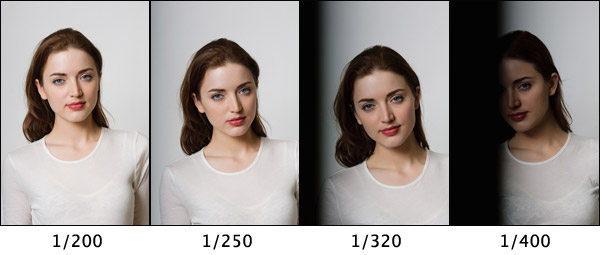
\includegraphics[width=1\textwidth]{./img/flash_unsync.jpg}\par
Source: http://neilvn.com/tangents/auto-fp-flash-setting-nikon-d300s-d700/ 
  \caption{Lack of synchronization between mechanical shutter and flash prevent parts of the image sensor from being exposed.}
  \label{fig:flash_unsync}
\end{figure}

As image sensor modules must be interchangeable, it is essential that the camera body is able to query each sensor's capabilities to ensure compatibility and sufficient performance in the parts of the design which are dependant on image format. Key capabilities are image resolution, video framerate, electronic shutter type (rolling or global) and bit depth. Additionally, image sensors use several different types of \glsp{cfa}, and so to be able to de-mosaic the image (interpolate RGB colour values), knowledge of the Bayer pattern used is required. For the image processor to be able to display colour images on the viewscreen it needs to be able to query the Bayer pattern type from the image sensor. 
 
Leading on from this, high-performance camera systems capture and store the raw greyscale output from the image sensor (hence the RAW format), avoiding in-camera image processing as much possible to ensure lossless image capture. \gls{dvi} only supports the RGB format and so needs extending to be able to transport high bit-depth RAW format data.
 
The technical details of each of these additions is described in the implementation part of this report.

\marginpar{Don't forget to reference this whole section to the DVI spec - once per paragraph}